\documentclass{CBM-PR-2020}
\usepackage{graphicx}
\usepackage[utf8]{inputenc}
\usepackage{amsmath}
\usepackage{amssymb}
\setlength{\titleblockheight}{35mm}

\begin{document}
\title{
Development and tests of readout chain for CBM Projectile Spectator Detector at FAIR
%\thanks{
%Work supported by XXX (Exchange XXX with your grant).
%}
}

\author[a]{D. Finogeev}
\author[a,b]{F. Guber}
\author[a]{N. Karpushkin}
\author[a,b]{A. Makhnev}
\author[a,c]{S. Morozov}
\author[a]{D. Serebryakov}

\affil[a]{Institute for Nuclear Research RAS, Moscow, Russia,}
\affil[b]{Moscow Institute of Physics and Technology, Dolgoprudny, Moscow Region, Russia}
\affil[c]{National Research Nuclear University MEPhI, Moscow, Russia}


%\author[1]{D. Finogeev, F. Guber, N. Karpushkin, A. Makhnev, S. Morozov, D. Serebryakov}
%\affil[1]{INR RAS, Moscow, Russia}

\maketitle

\section{PSD readout chain}


The PSD electronics architecture consists out of two major parts: a set of radiation-hard front-end boards and a readout rack, as shown in figure~\ref{fig:1} \cite {1}. Front-end boards are mounted directly onto The PSD modules, and are exposed to the particle flux generated by the experiment. Readout rack is located in a radiation-safe environment and is connected to the front-end part via 60m long signal cables.

\begin{figure}[htbp]
	\centering
	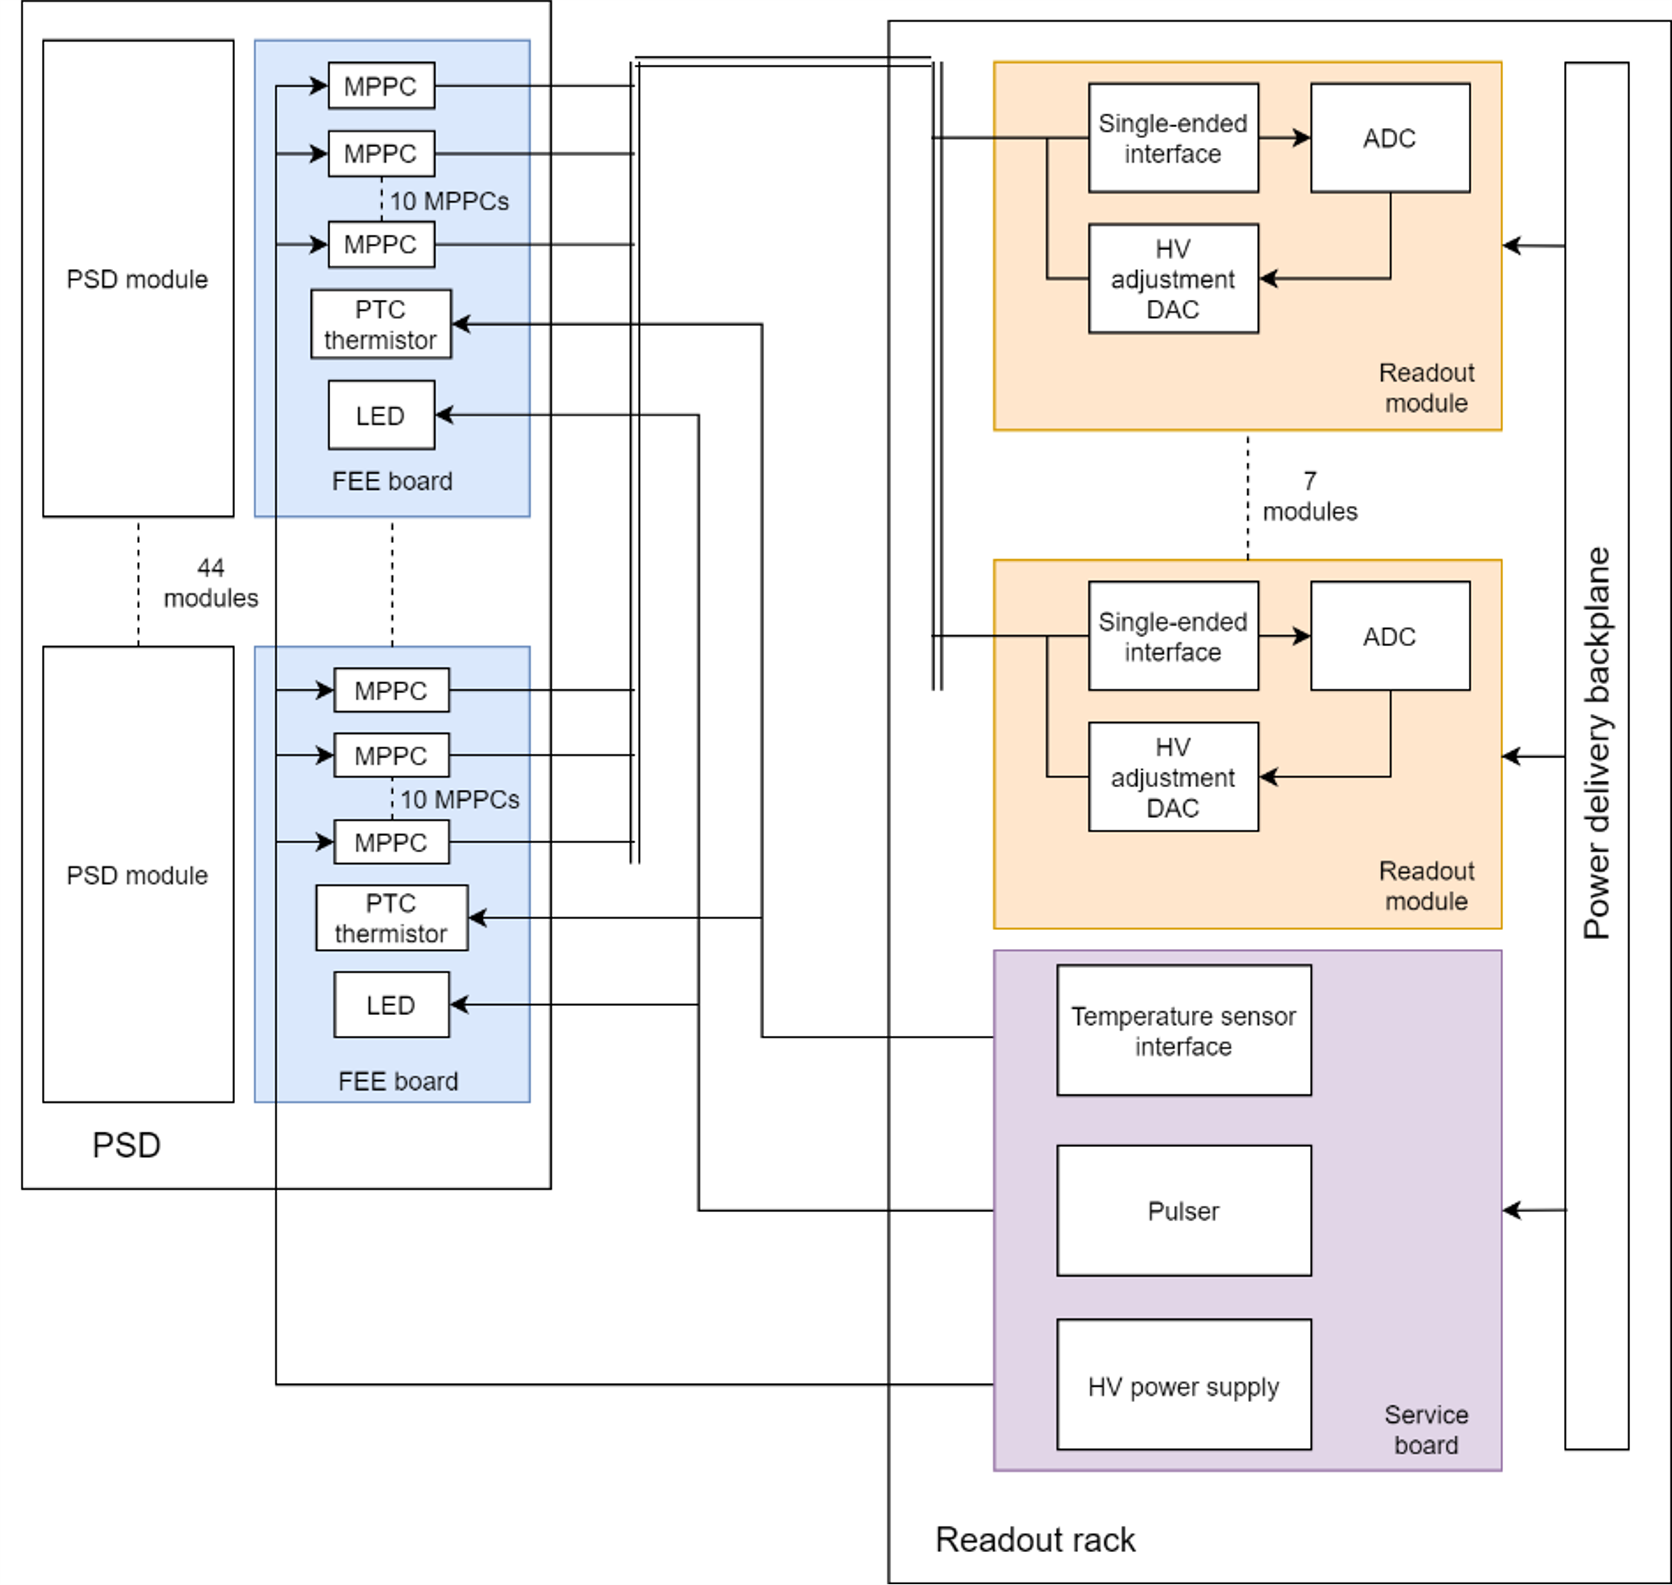
\includegraphics[width=.4\textwidth]{FEE_scheme.png}
	\caption{\label{fig:1} PSD electronics architecture diagram}
\end{figure}

The FEE boards are mounted directly onto PSD modules and host MPPCs, a temperature sensor (PTC thermistor), optical calibration LED, cable connectors and optical crosstalk protection hardware. These boards provide direct load of the MPPCs into 50 Ohm coaxial cables. FEE boards are fully designed assembled and tested on cosmic muons at mPSD setup in INR RAS, Moscow.

Readout module is an assembly of the ADC interface board and the ADC board itself. The ADC board initially designed for the ECAL detector of PANDA experiment \cite {2}. The 64-channel board is based on two Kintex 7 FPGA (field-programmable gate array) and LTM9011 ADC (analog-to-digital converter) with digitization rate up to 125Msps and 14-bit digitization resolution. To meet the requirements of CBM DAQ, GBT FPGA transceiver was integrated into the firmware. 

The ADC interface board and the ADC board are connected directly and are mounted together into the readout rack.
ADC interface board hosts single-ended to differential converters with adjustable input and output zero level, as well as high voltage correction circuit through common mode compensation: board may apply a DAC-controlled DC voltage onto a signal line, adjusting the common ~80V MPPC supply for each of the channels individually, leaving the AC signal unaffected. Both of the boards are designed and are in production. An evaluation version of the Readout module has been tested during beam tests runs at mCBM@SIS18 at the end of 2019 and beginning of 2020\cite{3}.


Service board is a multi-functional unit, designed to serve PSD needs, that are not related to the signal chain. Service board hosts a high voltage supply for biasing the MPPCs, as well as monitoring of the MPPCs current with automatic protection against overcurrent, temperature sensor interface through resistance-to-digital converters, optical calibration LED pulse generator and drivers. Operation of the board may be controlled directly through manual switches or remotely via a slow control interface.
An evaluation version of the Service board has been developed, manufactured and is undergoing verification and firmware development. Evaluation board may be easily scaled into a full-scale version.


\section{ The first mPSD beam test results at mCBM}
At the end of 2019 and beginning of 2020, beam tests at mCBM@SIS18 were carried out with Au and Pb ions at 1.01 - 1.22 AGeV energy range. Test of the mPSD prototype as a part of mCBM experiment allows to approve and verify the feasibility of the PSD readout concept. The prototype includes crucial parts of the readout such as Addon prototype board and ADC FPGA readout board. In this setup, Addon incorporated only the single-ended to differential converters and the necessary power systems. Photo of the assembled FEE setup is represented on figure~\ref{fig:4}.

\begin{figure}[htbp]
\centering % \begin{center}/\end{center} takes some additional vertical space
\raisebox{-0.5\height}{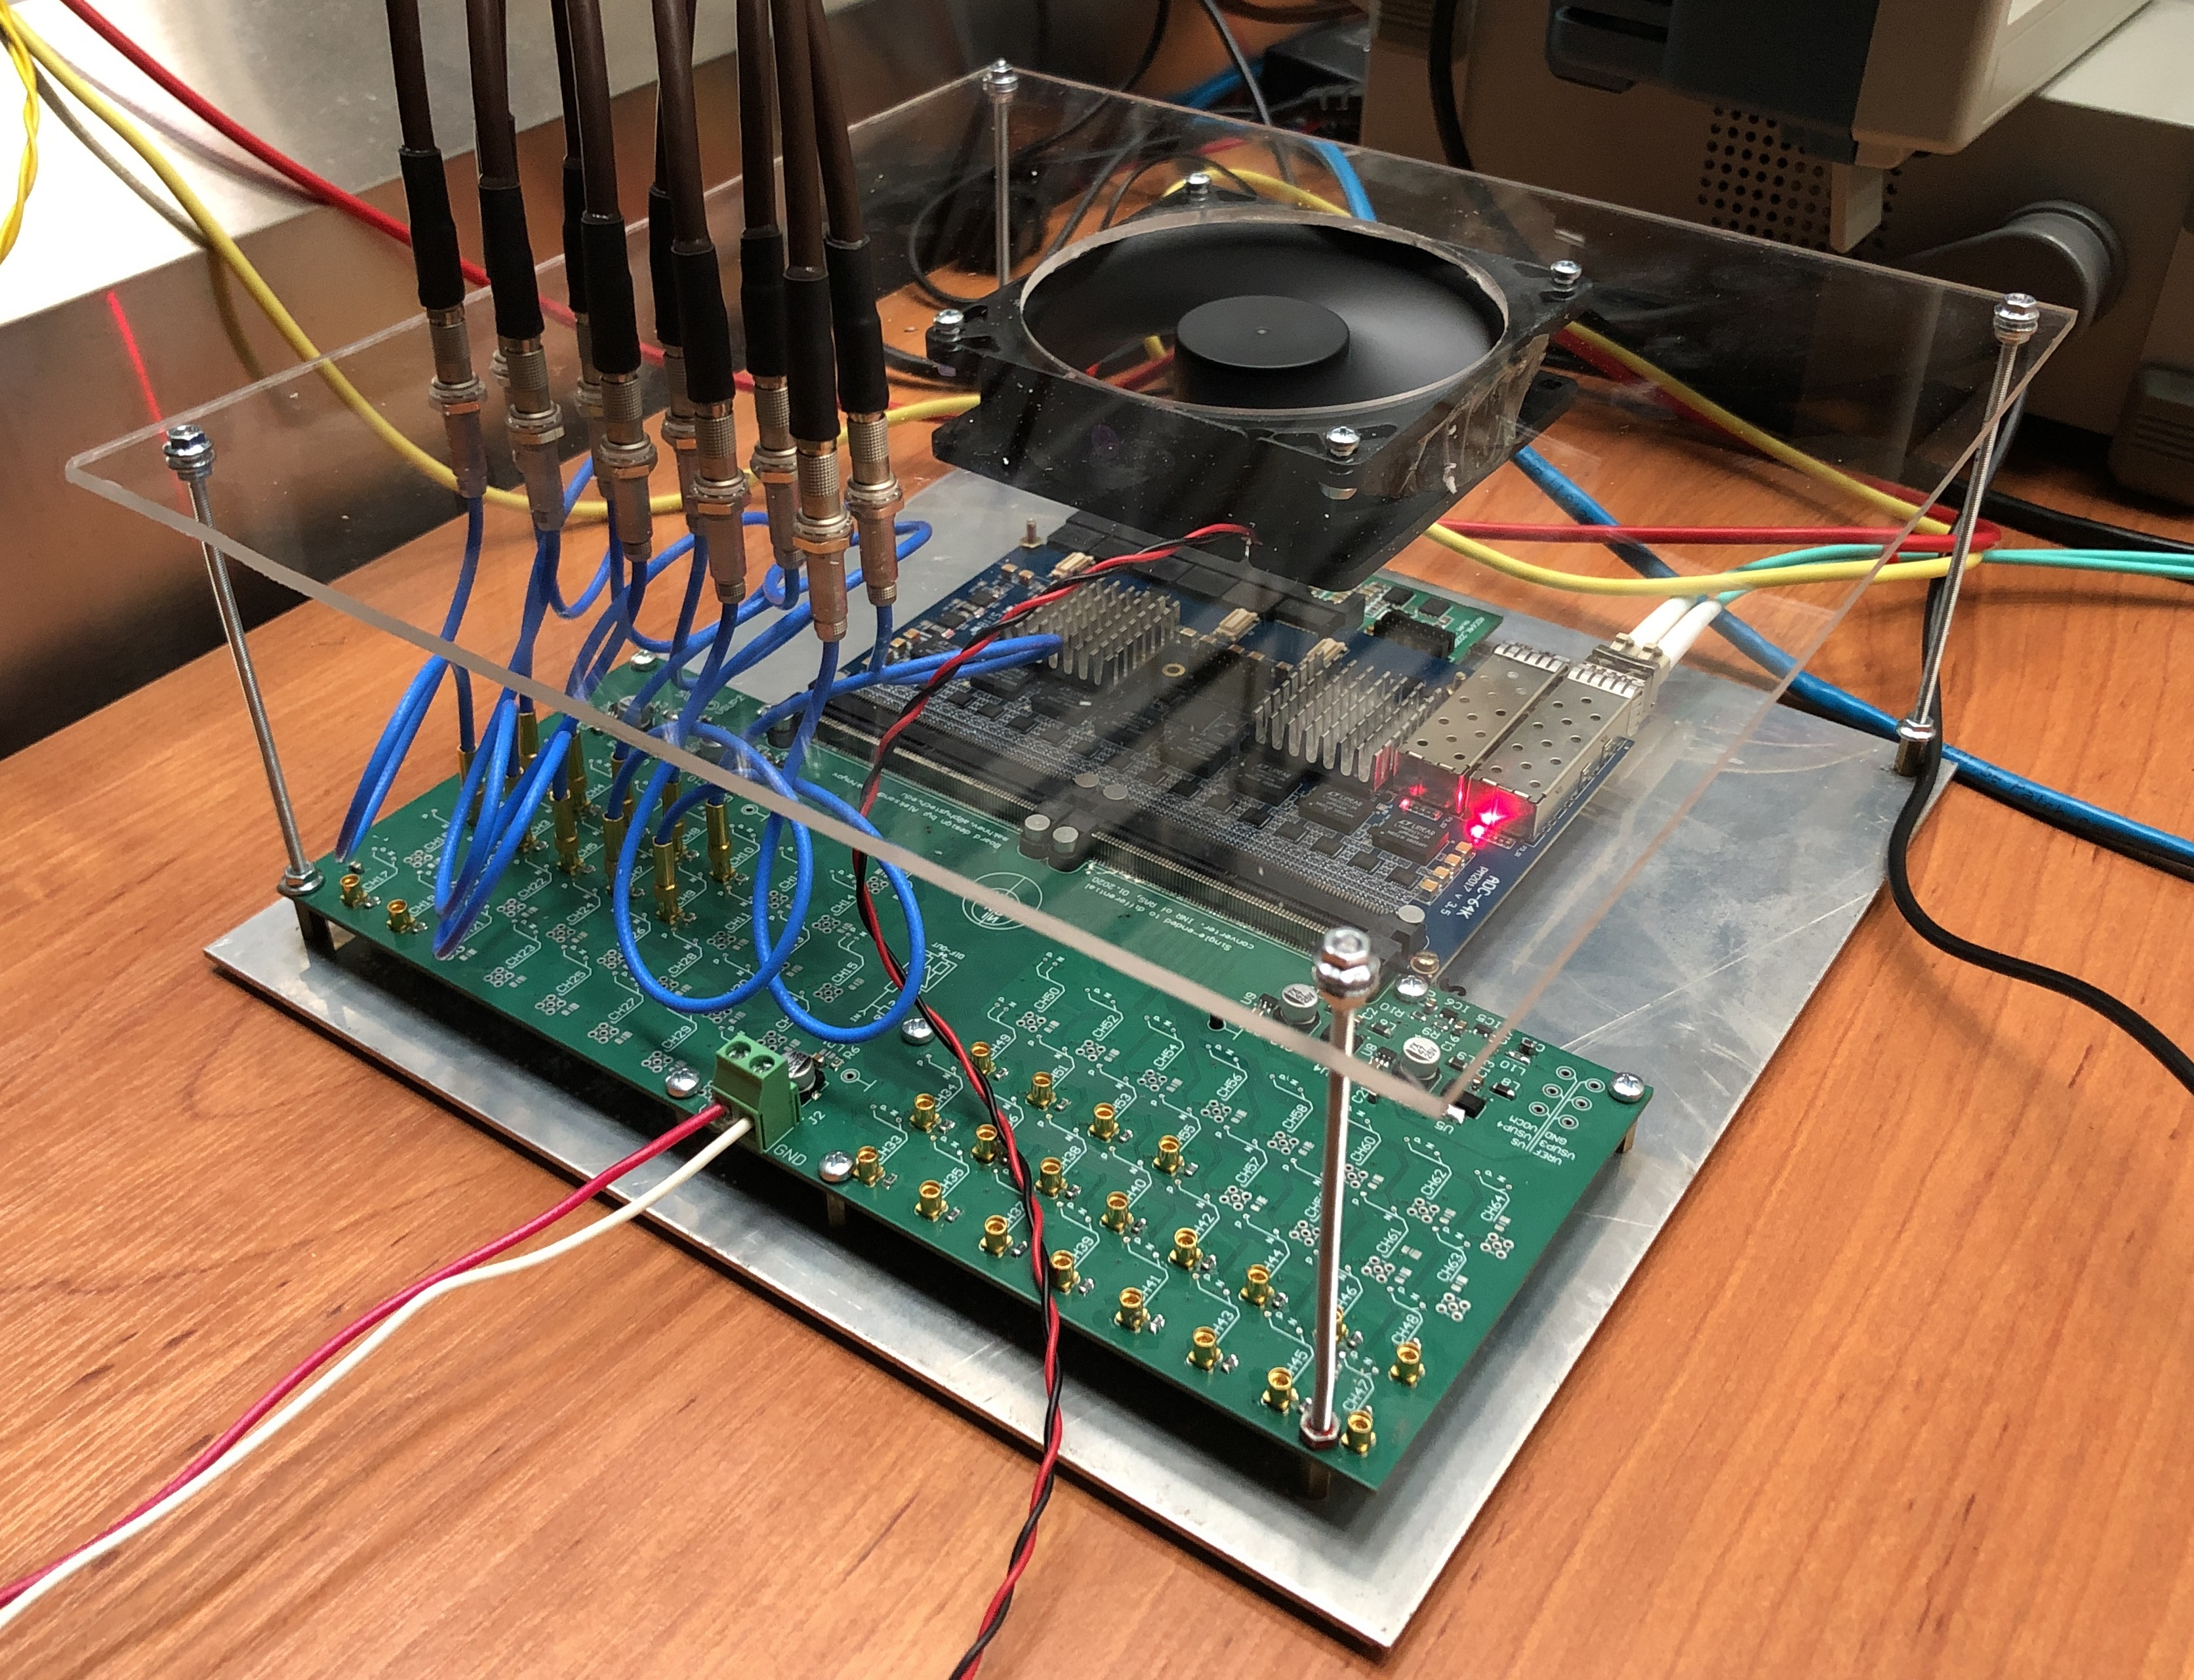
\includegraphics[width=.3\textwidth]{mPSD_FEE_photo.JPG}}
\qquad
\raisebox{-0.5\height}{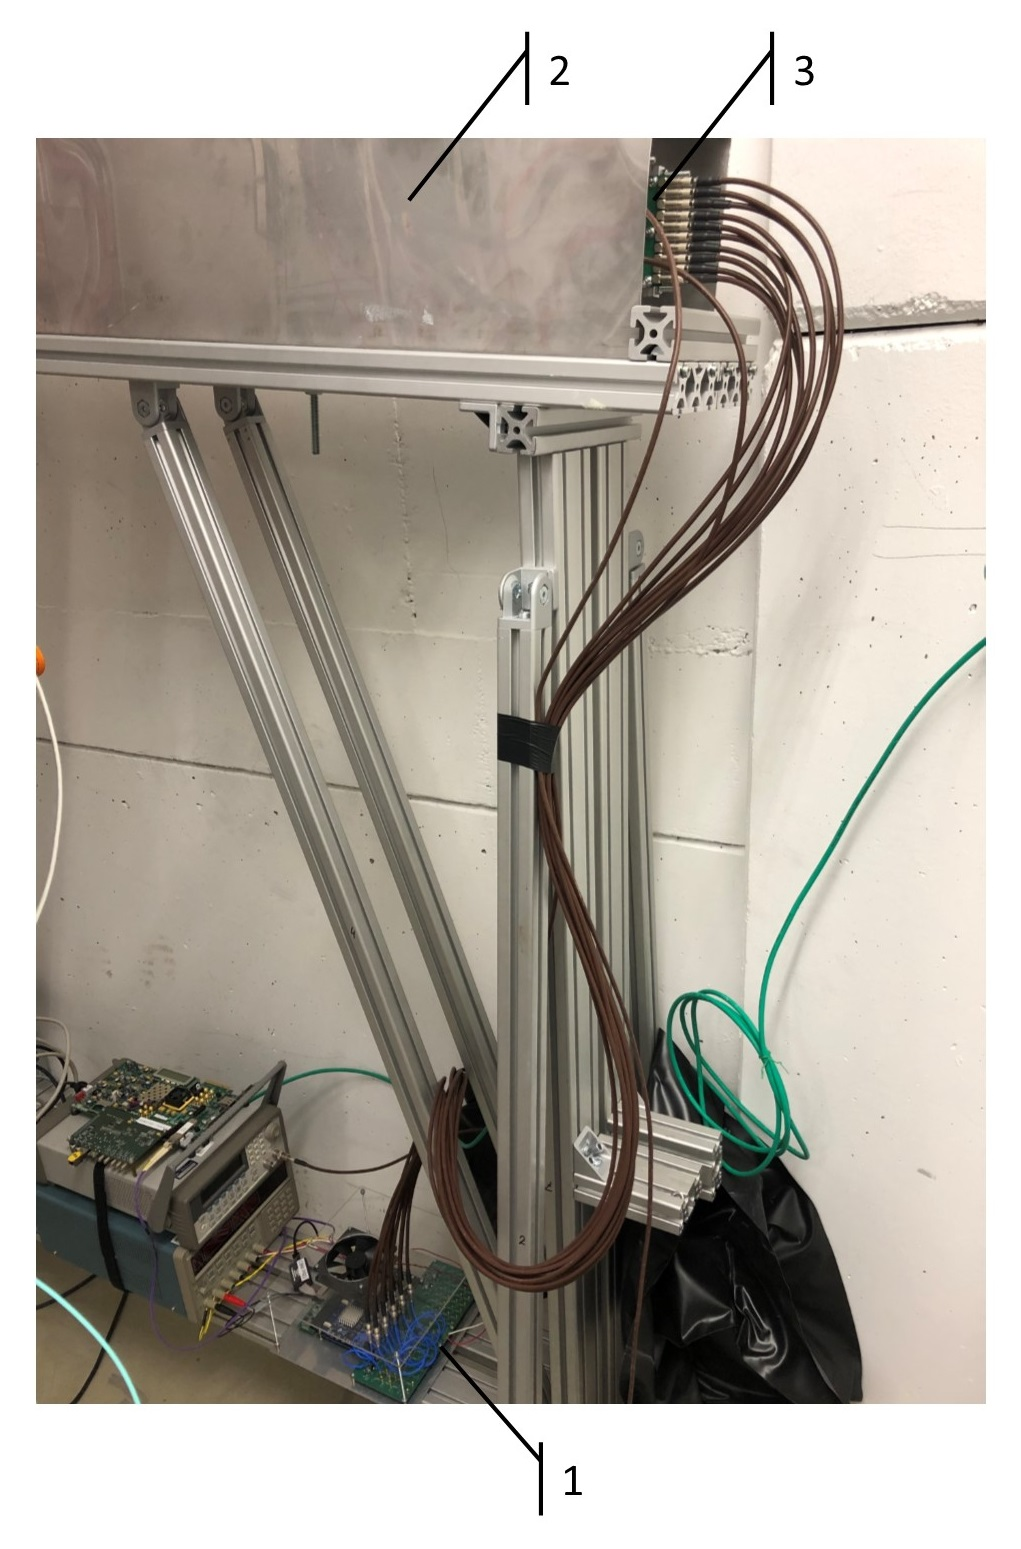
\includegraphics[width=.2\textwidth]{mPSD_module_photo.JPG}}
\caption{\label{fig:4} Photo of the ADC board assembled with the Addon board prototype (left); photo of mPSD module connected to FEE (right; 1 - Addon and ADC assembly, 2 - mPSD, 3 - MPPC board)}
\end{figure}

ADC FPGA board was connected to mCBM DAQ via GBT protocol used for data transport, clock distribution and configuration purposes. ADC was used in 80 Msps digitization mode. Each channel is triggered independently by amplitude threshold crossing and extracts data points from the waveform of the input signal measured in a fixed gate. ADC takes data in trigger-less readout mode according to CBM DAQ requirements. In addition, prototypes of all crucial software parts such as data unpacker, event building and data monitor were developed and tested.



\section{mPSD data monitoring}
Data from the mPSD detector read-out is transmitted to the mCBM common DAQ system using the DPB board with modified firmware. Currently, mPSD data consists of 64-bit frames containing information about the time stamp of the signal, total number and indices of triggered channels, integral of signal, zero levels and times of the signal's arrival, as well as the information about the signals waveforms.
The completeness and integrity of the received data packets is monitored by the number of read GBT words. In addition, control of all transmitted information is also carried out online through a software module developed for data monitoring (see figure~\ref{fig:5}). The top two graphs serve here to track the indices of triggered channels. The indices correspond to the mPSD sections from 0 to 8. An external source was connected to channel 9, which serves to check the synchronization between the mCBM detectors. The lower left graph shows the distribution of energy deposition in PSD sections. The major part of the energy is deposited in the two front sections of the calorimeter. The bottom right graph shows the evolution of the length of the microslices. This information is used to verify data integrity.

\begin{figure}[htbp]
\centering % \begin{center}/\end{center} takes some additional vertical space
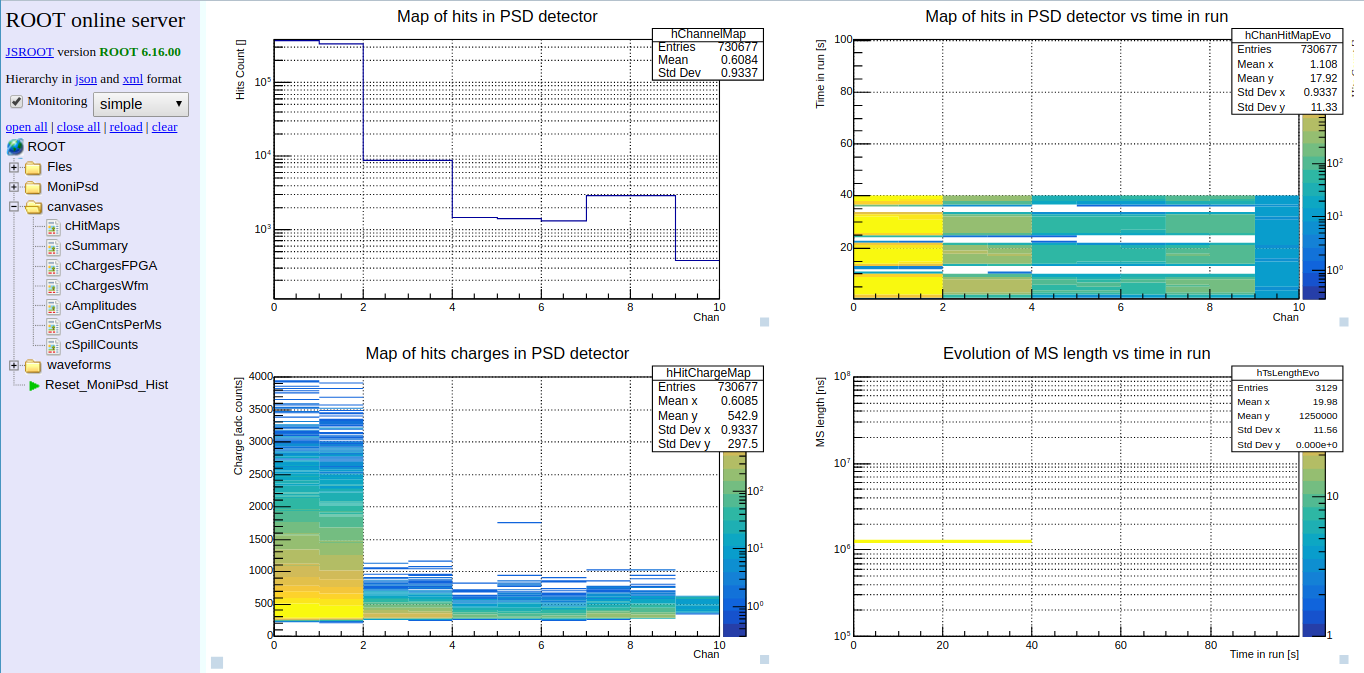
\includegraphics[width=\textwidth]{run582.png}
\caption{\label{fig:5} Data monitoring software module}
\end{figure}




\section{Preliminary mPSD test results}
One of the prime aims of mCBM is to test and validate the data processing concept and the reconstruction software which are being developed for the full CBM experiment. mCBM thus will be a demonstrator for the computing concept of CBM, including the reconstruction of events and selection of data in real-time and the full offline data analysis. It is thus planned to use already existing software components as far as possible for both online and offline computing in mCBM.
The challenge of the trigger-less readout is time synchronization and event building procedure. It is necessary to construct events from signals based on their time stamps while data processing.

\begin{figure}[htbp]
\centering % \begin{center}/\end{center} takes some additional vertical space
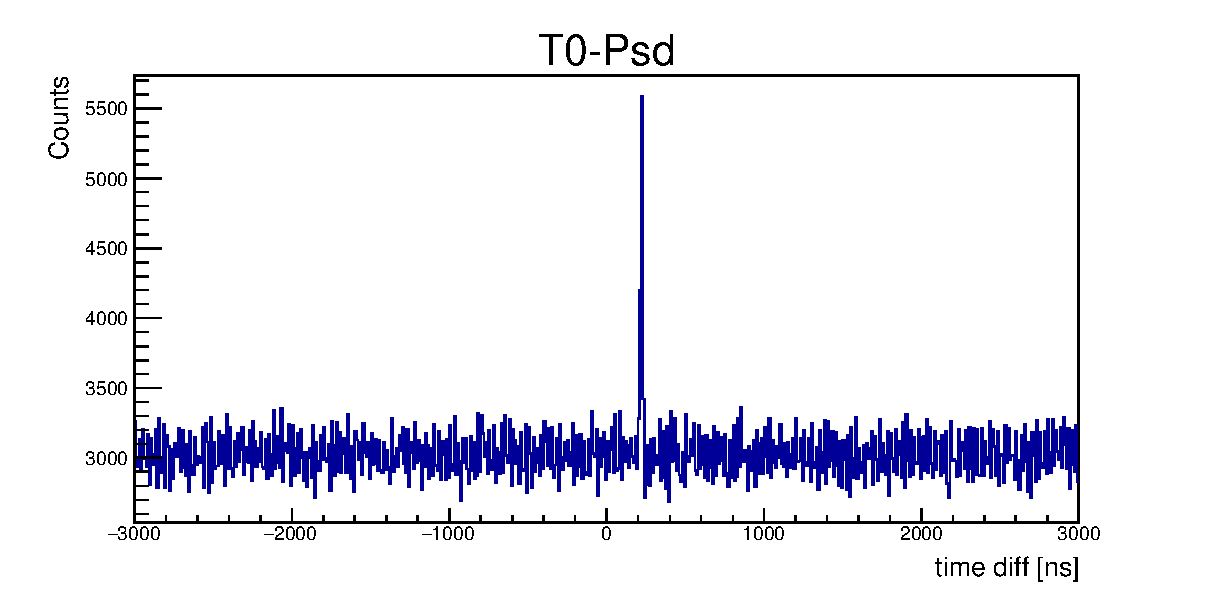
\includegraphics[width=.5\textwidth]{582_time_spectrum.eps}
\quad
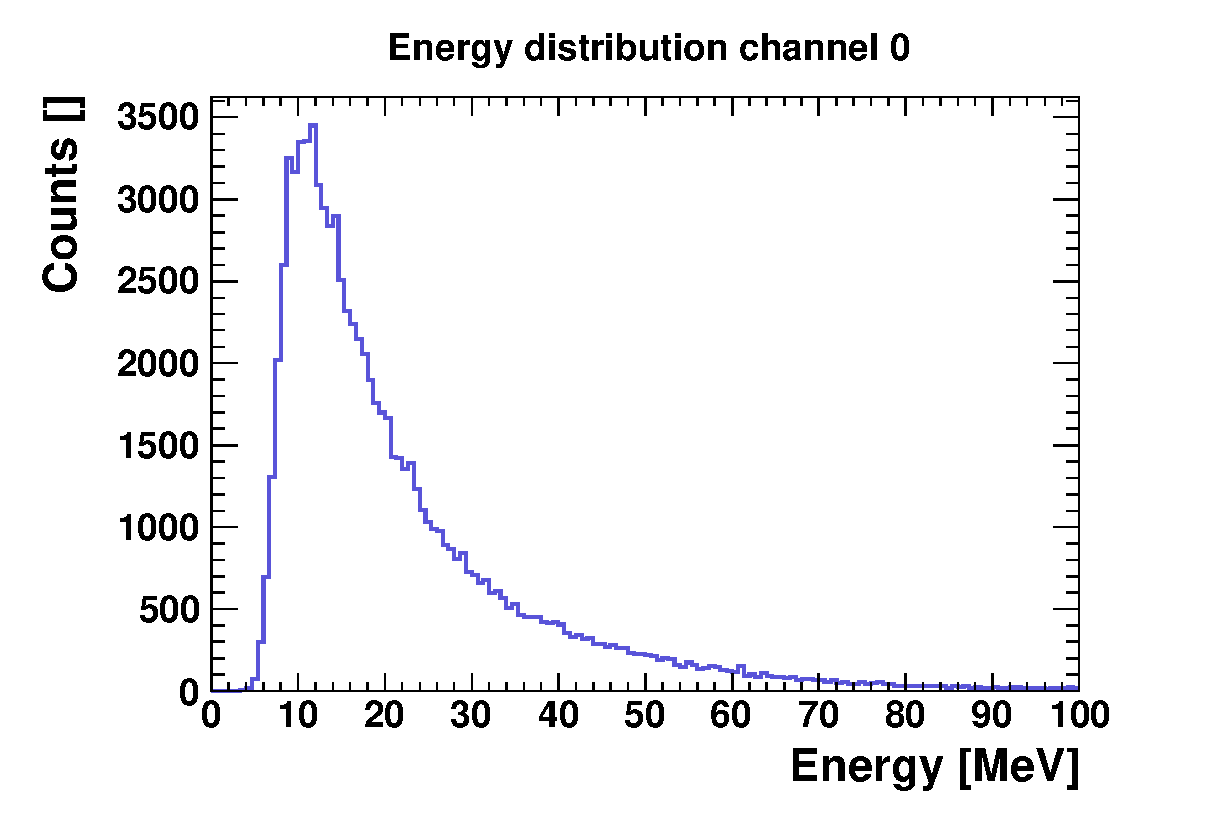
\includegraphics[width=.35\textwidth]{en_distrib_ch0.eps}
\caption{\label{fig:6} T0-Psd time correlation(left);  mPSD energy deposition in first section (right)}
\end{figure}




\begin{thebibliography}{9}   % Use for  1-9  references
\bibitem{1}
  D.~Finogeev, F.~Guber, N.~Karpushkin, A.~Makhnev, S.~Morozov and D.~Serebryakov,
  ``Development of readout chain for CBM Projectile Spectator Detector at FAIR,''
  J.\ Phys.\ Conf.\ Ser.\  {\bf 1690} (2020) no.1,  012059.
  doi:10.1088/1742-6596/1690/1/012059
  %%CITATION = doi:10.1088/1742-6596/1690/1/012059;%%
  
\bibitem{2}
Serneguet Sorli, Á. (2015). \emph{A multichannel digitizer for the PANDA experiment.} http://hdl.handle.net/10251/56722.

\bibitem{3}
Finogeev, D. et al., \emph{Readout system of the CBM Projectile Spectator                       Detector at FAIR} JINST 15 (2020) no.09, C09015
DOI: 10.1088/1748-0221/15/09/C09015


\end{thebibliography}


\end{document}

